\section{SPIQA (LLM)}
{{\footnotesize
\begin{description}[labelwidth=5em, labelsep=1em, leftmargin=*, align=left, itemsep=0.3em, parsep=0em]
  \item[date:] 2024-12-13
  \item[version:] TODO
  \item[last\_updated:] 2024-12
  \item[expired:] unknown
  \item[valid:] yes
  \item[valid\_date:] TODO
  \item[url:] \href{https://neurips.cc/virtual/2024/poster/97575}{https://neurips.cc/virtual/2024/poster/97575}
  \item[doi:] TODO
  \item[domain:] Multimodal Scientific QA; Computer Vision
  \item[focus:] Evaluating LLMs on image-based scientific paper figure QA tasks (LLM Adapter performance)
  \item[keywords:]
    - multimodal QA
    - scientific figures
    - image+text
    - chain-of-thought prompting
  \item[summary:] A workshop version of SPIQA comparing 10 LLM adapter methods on the SPIQA benchmark with scientific diagram/questions. Highlights performance differences between chain-of-thought and end-to-end adapter models.

  \item[licensing:] TODO
  \item[task\_types:]
    - Multimodal QA
  \item[ai\_capability\_measured:]
    - Visual reasoning
    - scientific figure understanding
  \item[metrics:]
    - Accuracy
    - F1 score
  \item[models:]
    - LLaVA
    - MiniGPT-4
    - Owl-LLM adapter variants
  \item[ml\_motif:]
    - Multimodal QA
  \item[type:] Benchmark
  \item[ml\_task:]
    - Multimodal QA
  \item[solutions:] TODO
  \item[notes:] Companion to SPIQA main benchmark; compares adapter strategies using same images and QA pairs.

  \item[contact.name:] Xiaoyan Zhong
  \item[contact.email:] unknown
  \item[results.links.name:] ChatGPT LLM
  \item[fair.reproducible:] Yes
  \item[fair.benchmark\_ready:] Yes
  \item[ratings.software.rating:] 0
  \item[ratings.software.reason:] Not analyzed.

  \item[ratings.specification.rating:] 6.0
  \item[ratings.specification.reason:] Task of QA over scientific figures is interesting but not fully formalized in input/output terms.

  \item[ratings.dataset.rating:] 6.0
  \item[ratings.dataset.reason:] Uses SPIQA dataset with \textasciitilde{}10 adapters; figures and questions are included, but not fully open.

  \item[ratings.metrics.rating:] 7.0
  \item[ratings.metrics.reason:] Reports accuracy and F1; fair but no visual reasoning-specific metric.

  \item[ratings.reference\_solution.rating:] 6.0
  \item[ratings.reference\_solution.reason:] 10 LLM adapter baselines; results included.

  \item[ratings.documentation.rating:] 5.0
  \item[ratings.documentation.reason:] Poster paper and limited documentation; no reproducibility instructions.

  \item[id:] spiqa\_llm
  \item[Citations:] \cite{pramanick2025spiqadatasetmultimodalquestion}
  \item[Ratings:]
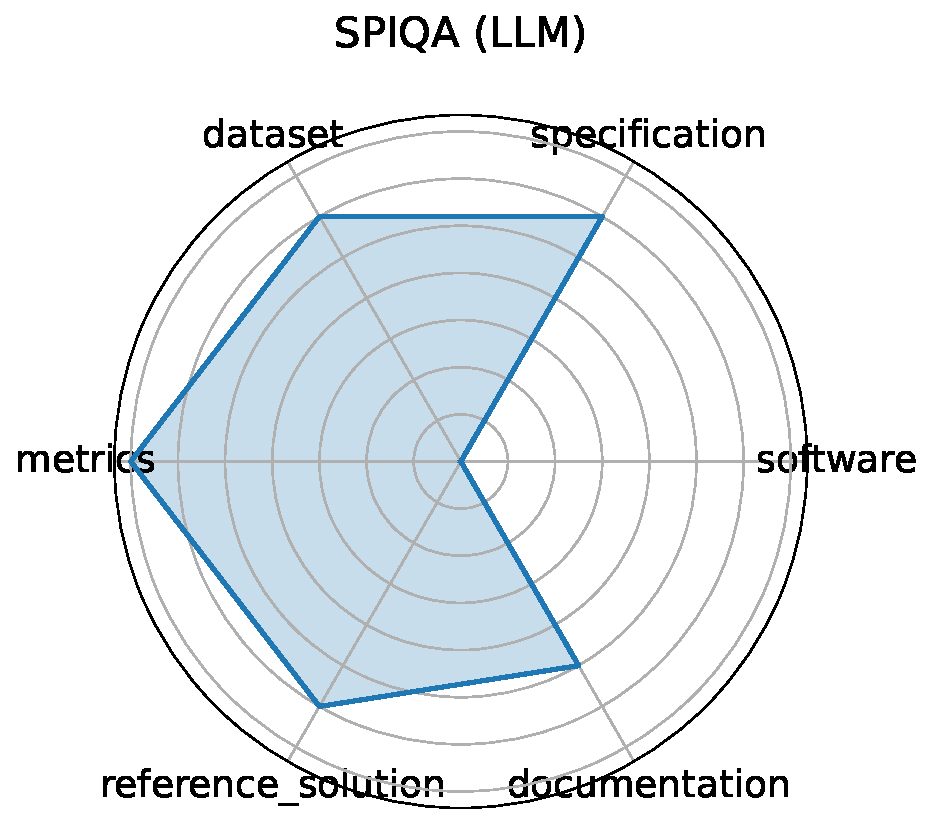
\includegraphics[width=0.2\textwidth]{spiqa_llm_radar.pdf}
\end{description}
}}
\clearpage